\chapter{関連研究}
\label{chap:previousworks}
本章では\secref{sec:generate_animation}で音からアニメーションを自動生成する研究を紹介し,\secref{sec:generate_}でアニメーションから音を自動生成する研究を紹介する.
\secref{sec:synchronization}では音とアニメーションを同期させる研究,
\secref{sec:marching}で本論文と同様,吹奏楽に関連した研究を紹介し,最後に\secref{sec:compere}にて本研究の新規性を述べる.

\section{音からアニメーションを自動生成する研究}\label{sec:generate_animation}
音とアニメーションを同期させることを目的として,音からアニメーションを自動生成する研究は多く存在している.\\
\indent
物が落下するアニメーションを生成するには,物の落下音と物が落下するタイミングを1つ1つ合わせる必要がある.
Langloisら\cite{IFA}は,それらを正確に合わせるために,物が落下する音が収録されている音源から,物が落下するアニメーションを自動生成する手法を提案した.\\
%\begin{figure}[h]
%	\centering
%	
\includegraphics[width=15cm]{fig/chap2/IFA.eps}
%	\caption{落下アニメーションの自動生成結果}
%	\label{fig:IFA}
%\end{figure}
%
\indent
キャラクタの口の動きと音声を合わせる,リップシンクも難しい課題となっている.
キャラクタの口の動きに合わせて後から音声を録音するアフレコは比較的容易であるが,音声から,その言葉を発している口元のアニメーションの生成は,言葉と口の形,そして発するタイミングと口の動きを合わせる必要があり,ひじょうに難易度が高い.
そこで,Edwardsら\cite{JALI}は,台詞が収録されている音源および台詞が記載されているテキストファイルを入力すると,その台詞を話している口元のアニメーションを自動生成する手法を提案した.
本手法では,顎と唇だけを制御することにより,自然な口元のアニメーションを自動生成している.更に,後から表情を編集することが可能となっているため,最終的には自然な表情のアニメーションが完成する.\\
%\begin{figure}[h]
%	\centering
%	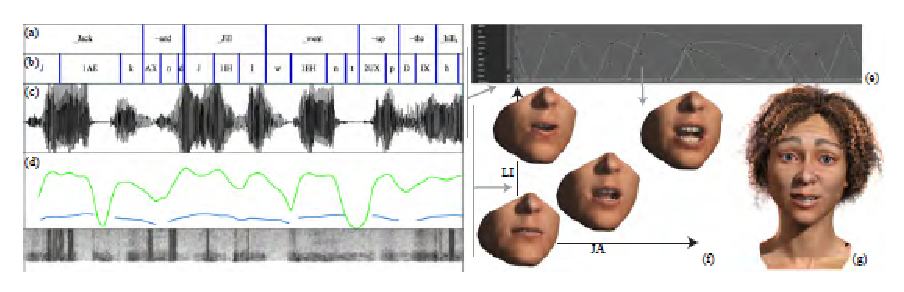
\includegraphics[width=15cm]{fig/chap2/JALI.eps}
%	\caption{口元アニメーションの自動生成}
%	\label{fig:JALI}
%\end{figure}
%
\indent
本論文の目的と同じように,音源から楽器を演奏するアニメーションを自動生成する研究も多く行われている.
Zhuら\cite{piano}は,MIDI音源からピアノを弾く指元のアニメーションを自動生成する手法を提案した.
ピアノのような楽器は,指と音が1体1で対応していないため,フレーズにより指使いを変える必要がある.
ある指が他の指の上や下を通るような指使いの時は,指同士が衝突しないように考慮する必要もある.
彼らの手法では,これらの課題を解消することが可能である.
%\begin{figure}[h]
%	\centering
%	
\includegraphics[width=15cm]{fig/chap2/piano.eps}
%	\caption{ピアノを弾く手元のアニメーションの自動生成}
%	\label{fig:piano}
%\end{figure}
%
\section{アニメーションから音を生成する研究}\label{sec:generate_sound}
音とアニメーションを同期させることを目的として,物理シミュレーションの結果を音に反映させる研究分野が存在する.\\
%
\subsection{サウンドレンダリング}
サウンドレンダリングという分野は,物理アニメーションを生成すると同時に音を生成することにより,双方を同期させることを目的とする分野である.
CG-ARTSの教育リポート,『音を描き出す夢の実現』\cite{CG-ARTS}によると,本分野は1990年代前半に登場し,未だ実験的にとどまっている分野となっている.
2009年には1つのシミュレーションパイプラインの中で,CGアニメーションと,それに呼応した音を同時に生成するアルゴリズム\ref{james1}が考案された.
本アルゴリズムはZhengらにより考案され,水が流れる様子を再現したアニメーションと音の見事な同期が達成された.
%\begin{figure}[h]
%	\centering
%	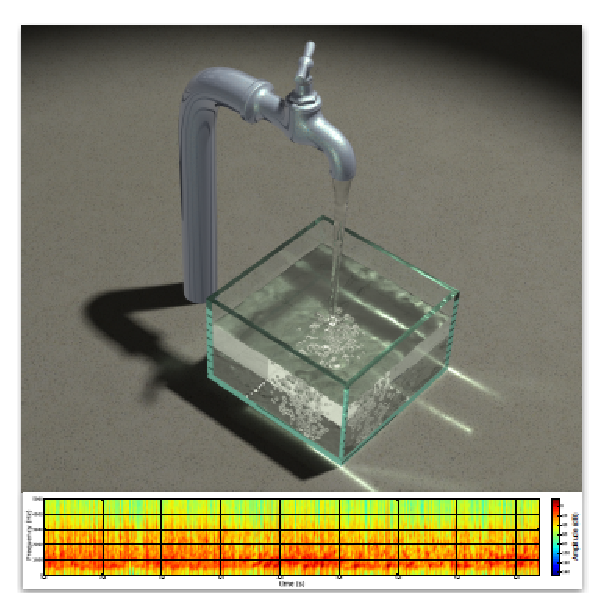
\includegraphics[width=15cm]{fig/chap2/james1.eps}
%	\caption{水のアニメーションと音の同時生成結果}
%	\label{fig:james1}
%\end{figure}
%
翌年には,同氏らにより破壊音を自動生成するアルゴリズム\cite{james2}が発表された.
本アルゴリズムでは,さまざまな剛体の破壊音だけでなく,その衝撃が間接的におよぼす影響も考慮されているため,\figref{fig:james2}のような複数の物体がぶつかり,破壊されるような複雑なシーンでも,忠実に音が再現された.
\begin{figure}[h]
	\centering
	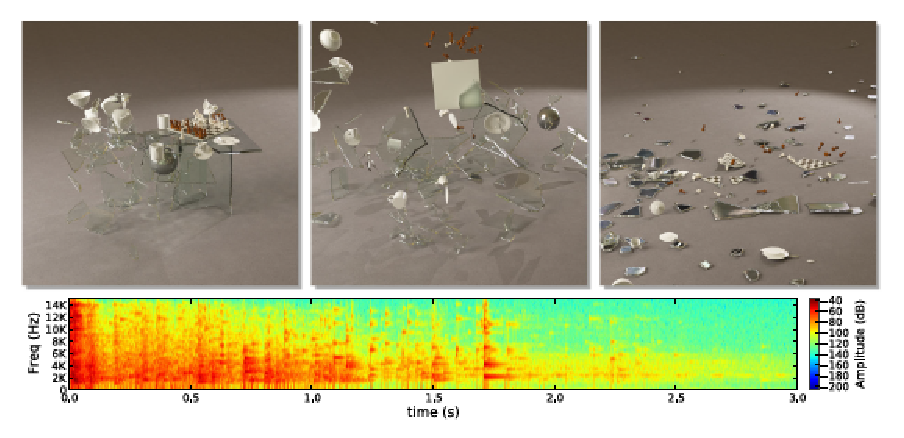
\includegraphics[width=14cm]{fig/chap2/james2.eps}
	\caption{複数の剛体がぶつかり破壊される様子}
	\label{fig:james2}
\end{figure}

\subsection{プロシージャルオーディオ}
アニメーションから音を自動生成する技術は,ゲームのような,使用可能なメモリが限られている場合には,できる限りメモリを節約したい.
ゲームソフトを開発している株式会社スクウェア・エニックスは,メモリを節約するため,プロシージャルという技術を研究している.
この技術は2014年のCEDEC\cite{SQUARE}にて発表されており,あらかじめ作っておいた音をゲーム内で使用するのではなく,音をプログラムで作り出す技術をさす.
ゲームでは,プレイヤの操作に合わせて音を鳴らすタイミングを内部で調節する必要がある.
そのことからも,この技術はゲームにおいて特に必要な技術であると考えられる.

\section{音とアニメーションを同期させる研究} \label{sec:synchronization}
片方からもう一方を自動生成する研究だけでなく,既に生成されている双方を編集することにより同期させる研究も存在する.
Leeら\cite{Lee}は,MIDI音源およびキャラクタのモーションデータを入力とし,双方を最小限編集することにより,MIDI音源と同期したキャラクタのダンスアニメーションを生成する手法を提案した.\\
%\begin{figure}[h]
%	\centering
%	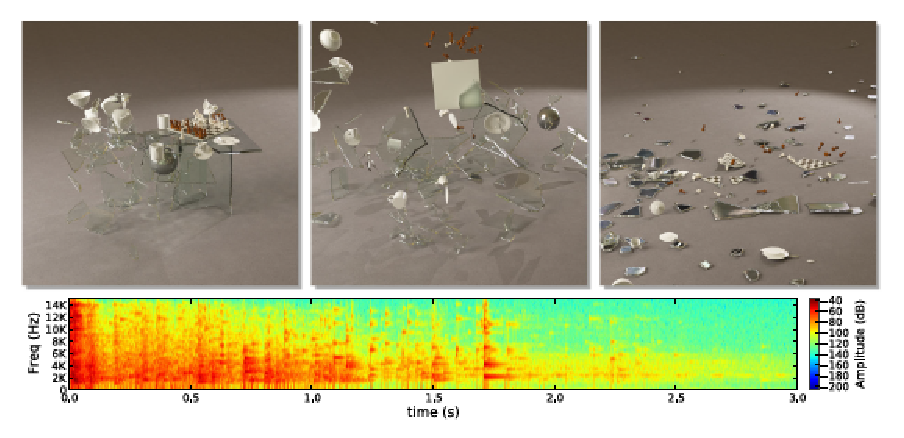
\includegraphics[width=15cm]{fig/chap2/james2.eps}
%	\caption{ダンスアニメーションと音を同期}
%	\label{fig:lee}
%\end{figure}
\indent
このような研究は,複数のカットを組み合わせて作成する,モンタージュの作成にも応用されている.
Liaoら\cite{Liao}は,BGMとなる音源および複数のビデオクリップを入力することにより,BGMに合ったモンタージュを作成する手法を提案した.

\section{マーチングを行う演奏者の軌跡を解析する研究} \label{sec:marching}
マーチングとは,演奏者が演奏しながら定められた経路に従って歩くことにより隊形を作る,吹奏楽の演奏形態である.
本論文の筆者は,マーチングを行う1人の演奏者に注目し,その演奏者が歩くべき経路と実際の経路の誤差を表示するシステム\figref{fig:marching}を提案した.
本システムにより,演奏者は自身の歩行の改善点を知ることができ,その結果マーチングの隊形の完成度を高めることが期待できる.
\begin{figure}[h]
	\centering
	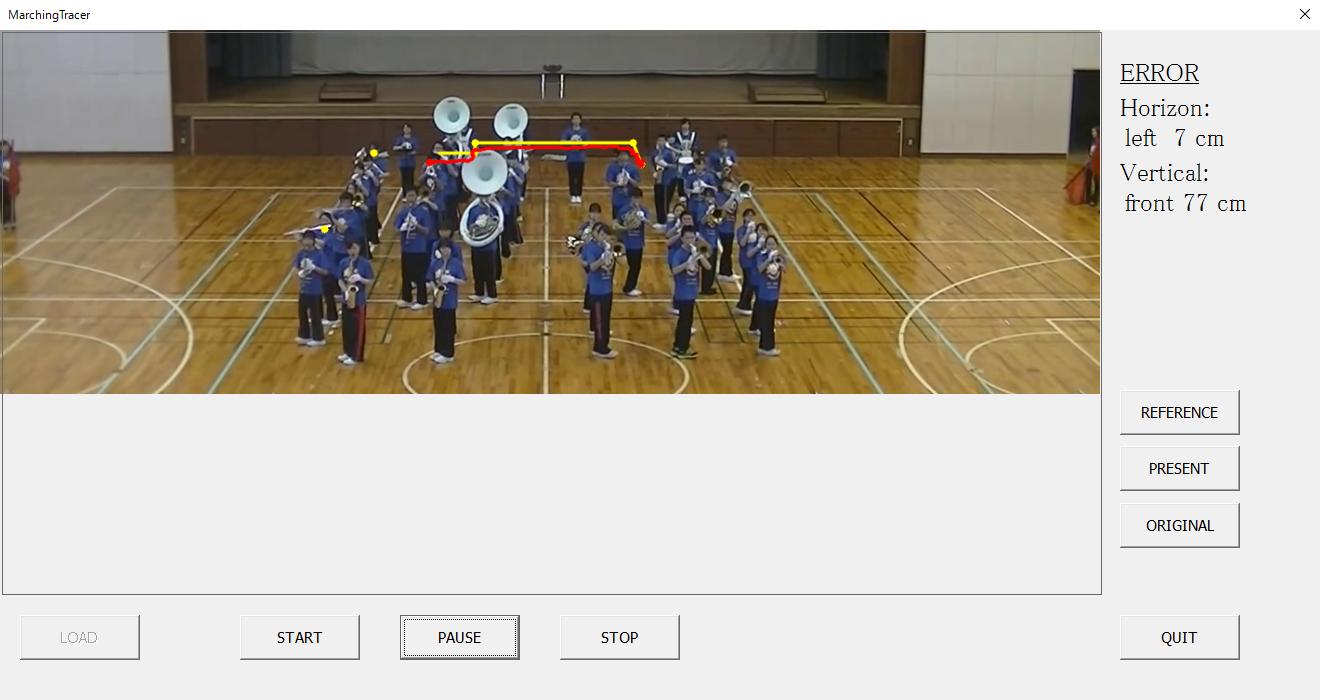
\includegraphics[width=14cm]{fig/chap2/marching.eps}
	\caption{マーチングを行う演奏者の軌跡および誤差の表示例}
	\label{fig:marching}
\end{figure}
なお,本研究の成果はNICOGRAPH2016にてポスター発表\cite{NICOGRAPH}を行った.
そして,一連の研究をまとめた成果が画像電子学会誌のVol.47\cite{iieej}に掲載される予定である.

\section{本研究の新規性}\label{sec:compere}
アニメーションと音の同期や,吹奏楽をテーマとした研究は多く存在する.
しかし,管楽器を演奏するキャラクタと音の同期に注目した研究は存在しない.
したがって本研究の新規性は,管楽器を演奏するアニメーションを,音から自動生成するという点である.
さらに,本論文ではトランペット奏者およびトロンボーン奏者に適用した例だけを示すが,音と指使いの対応表を用意することにより,すべての管楽器の演奏アニメーションが入力音源から自動生成が可能である.
このように,あらゆる楽器への対応が可能である点も新規性である.